\documentclass[../main.tex]{subfiles}

\begin{document}
        
    \chapter{Ramsay-Cass-Koopmans Model}
        
        Growth rates of technology and labor (also population) remain exogenous and constant as in Solow model,
        \begin{align}
            \frac{\dot A(t)}{A(t)} = g, \quad \frac{\dot L(t)}{L(t)} = n
            \implies
            A(t) = A(0)e^{gt}, \quad L(t) = L(0)e^{nt}
        \end{align}
        However, law of motion of capital is determined by \textbf{optimizing} households (with no depreciation of capital):
        \begin{align}
            \dot K(t) = Y(t) - \zeta(t),
        \end{align}
        where $\zeta(t) = C(t)L(t)$ is the aggregate consumption in the economy.
        
    \section{Firms}
    
        Representative firm has homogeneous of degree one production function,
        \begin{align}
            Y = F (K, A L),
            \quad
            F(c K, c A L)
            = c F(K, A L)
        \end{align}
        
        where $K(t), A(t), L(t)$ are capital, technology and labor. Output per effective labor is then
        \begin{align}
            y
            = \frac{F(K, AL)}{AL}
            = F\left(\frac{K}{AL}, 1\right)
            = f(k)
            \quad s.t. \quad f'(k) > 0,\; f''(k) < 0.
        \end{align}
        
        Firms continuously maximize instantaneous profit by choosing capital and labor
        \begin{align}
            \max_{K(t), L(t)} \Pi(t)
            = F(K, A L) - [r K + W L ]
        \end{align}
        
        where $r(t)$ is the interest rate and $W(t)$ is wage rate. With FOC with respect to $K(t)$, we have that
        \begin{align}
            \frac{\partial \Pi(t)}{\partial K(t)}  = 0
            \implies
            r(t)
            = \frac{\partial F(K, AL)}{\partial K}
            &= AL \frac{\partial F\left(\frac{K}{AL}, 1\right)}{\partial K}
            \\
            &= AL
            \frac{\partial f(k)}{\partial K}
            = AL
            \underbrace{\frac{\partial f(k)}{\partial k}}_{f'(k)}
            \underbrace{\frac{\partial k}{\partial K}}_{1/(AL)} = f'(k)
            \\
            \implies
            r(t) &= f'(k),
            \label{eqn:rck-eqm-interest}
        \end{align}
        which is the equilibrium interest rate. With FOC with respect to $L(t)$, we have
        \begin{align}
            \frac{\partial \Pi(t)}{\partial L(t)}  = 0
            \implies
            W(t)
            = \frac{\partial F(K, AL)}{\partial L}
            &= \left[\frac{\partial F(K, AL)}{\partial AL}\right]
            \frac{\partial AL}{\partial L}
            \\
            &= A \left[\frac{\partial AL \cdot f(k)}{\partial AL}\right]
            = A f(k) + A
            \underbrace{\frac{\partial f(k)}{\partial k}}_{f'(k)}
            \underbrace{\frac{\partial k}{\partial AL}}_{-\frac{k}{AL}}
            \\
            \implies
            W(t) &= A [f(k) - k f'(k)]
            \\
            \implies
            \frac{W(t)}{A(t)} = w(t)
            &= f(k) - k f'(k)
            \label{eqn:rck-eqm-wage}
        \end{align}
        
        which is the equilibrium wage per effective labor.
        
    \section{Households}
        
        Each of $H$ identical households chooses consumption to maximize present value of utility:
        \begin{align}
            \max_{C(t)} U
            &= \int_{t=0}^\infty e^{-\rho t} u(C(t)) \frac{L(t)}{H} dt
            \label{eqn:rck-pv}
            \\
            &  s.t. \nonumber
            \\
            \int_{t=0}^\infty e^{-R(t)} C(t) \frac{L(t)}{H} dt
            &\le
            \frac{K(0)}{H} + \int_{t=0}^\infty e^{-R(t)} W(t) \frac{L(t)}{H} dt
            \label{eqn:rck-bc}
        \end{align}
        
        where $C(t)$ is consumption per worker, $\rho$ is the time discount rate and $R(t) = \int_{\tau=0}^t r(\tau) d \tau$ accounts for continuous compounding interest. We can rewrite the budget constraint in \eqref{eqn:rck-bc} as
        \begin{align}
            \lim_{s\to\infty}
            \left[\frac{K(0)}{H} + \int_{t=0}^s e^{-R(t)} \left[W(t) - C(t)\right] \frac{L(t)}{H} dt\right]
            &\ge 0
        \end{align}
        
        Household wealth at time $s$ is then
        \begin{align}
            \frac{K(s)}{H}
            &= e^{R(s)}
            \left[ \frac{K(0)}{H} + \int_{t=0}^s e^{-R(t)} \left[W(t) - C(t)\right] \frac{L(t)}{H} \right]
            \\
            \implies
            \lim_{s\to\infty} e^{-R(s)} \frac{K(s)}{H}
            &= \lim_{s\to\infty} 
            \left[ \frac{K(0)}{H} + \int_{t=0}^s e^{-R(t)} \left[W(t) - C(t)\right] \frac{L(t)}{H} \right]
            \\
            \implies
            \lim_{s\to\infty} e^{-R(s)} \frac{K(s)}{H} &\ge 0.
            \label{eqn:no-ponzi}
        \end{align}
        Equation \eqref{eqn:no-ponzi} is called the \textbf{no ponzi-game condition}, imposing that present value of assets cannot be negative in the limit.
        
        \vspace{0.5cm}
        
        Let $c(t) = \frac{C(t)}{A(t)}$ be consumption per effective labor, and assume CRRA instantaneous utility function. Since $A(t) = A(0) e^{gt}$ and $L(t) = L(0)e^{nt}$, we rewrite objective function \eqref{eqn:rck-pv} as
        \begin{align}
            U &= \int_{t=0}^\infty
            e^{-\rho t}
            \frac{C(t)^{1-\theta}}{1-\theta}
            \frac{L(t)}{H} dt,
            \quad \theta > 0
            \\
            &= \int_{t=0}^\infty
            e^{-\rho t}
            \left[A(0)^{1-\theta} e^{(1-\theta)gt}\frac{c(t)^{1-\theta}}{1-\theta}\right]
            \frac{L(0)e^{nt}}{H} dt
            \\
            &= B \int_{t=0}^\infty e^{-\beta t}
            \frac{c(t)^{1-\theta}}{1-\theta} dt
            \label{eqn:rck-pv2}
        \end{align}

        where $B = A(0)^{1-\theta}\frac{L(0)}{H}$ and $\beta = \rho - n - (1-\theta)g > 0$. Rewrite \eqref{eqn:rck-bc} as 
        \begin{align}
            & \frac{K(0)}{H} + \int_{t=0}^\infty e^{-R(t)} [W(t) - C(t)] \frac{L(t)}{H} dt
            \ge 0
            \\
            \implies&
            k(0)\frac{A(0) L(0)}{H}
            + \int_{t=0}^\infty e^{-R(t)} [w(t) - c(t)] \frac{A(t) L(t)}{H} dt
            \ge 0
            \\
            \implies&
            k(0)\frac{A(0) L(0)}{H}
            + \int_{t=0}^\infty e^{-R(t)} [w(t) - c(t)] e^{(g + n)t}\frac{A(0) L(0)}{H} dt
            \ge 0
            \\
            \implies&
            k(0) + \int_{t=0}^\infty e^{-R(t) + (g + n)t} [w(t) - c(t)] dt
            \ge 0
        \end{align}
        
        Forming the Lagrangian,
        \begin{align}
            \L
            = B \int_{t=0}^\infty e^{-\beta t}
            \frac{c(t)^{1-\theta}}{1-\theta} dt
            + \lambda
            \left(
            k(0) + \int_{t=0}^s e^{-R(t) + (n+g)t} \left[w(t) - c(t)\right]
            \right)
        \end{align}
        we have with FOC with respect to $c(t)$ that
        \begin{align}
            \frac{\partial \L}{\partial c(t)} = 0
            % &\implies
            % B e^{-\beta t} c(t)^{-\theta} = e^{-R(t) + (n+g)t}
            % \\
            & \implies
            B c(t)^{-\theta} = e^{-R(t) + (n + g + \beta)t}
            % \\
            % & \implies
            % \ln B -\theta \ln c(t) = -R(t) + (n + g + \beta)t
            \\
            & \implies
            \frac{d}{dt}\left(\ln B -\theta \ln c(t)\right)
            = \frac{d}{dt} \left( -R(t) + (n + g + \beta)t \right)
            \\
            & \implies
            -\theta \frac{\dot c(t)}{c(t)}
            = -r(t) + (n + g + \left[\rho - n - (1-\theta) g\right])
            \\
            & \implies
            \frac{\dot c(t)}{c(t)}
            = \frac{r(t) - \rho - \theta g}{\theta}.
            \label{eqn:consumption-path}
        \end{align}
        
        Equation \eqref{eqn:consumption-path} is the optimal consumption path, which can also be expressed in $C(t)$ as
        \begin{align}
            C(t) = A(t) c(t) \implies
            \frac{\dot C(t)}{C(t)}
            = \frac{\dot A(t)}{A(t)} + \frac{\dot c(t)}{c(t)}
            = g + \frac{r(t) - \rho - \theta g}{\theta} = \frac{r(t) - \rho}{\theta}.
        \end{align}
        
        
    \section{Dynamics of model}
        
        From optimal consumption path \eqref{eqn:consumption-path} and equilibrium interest \eqref{eqn:rck-eqm-interest}, we have on the \textbf{balanced growth path (BGP)} that
        \begin{align}
            \frac{\dot c(t)}{c(t)}
            = \frac{r(t) - \rho - \theta g}{\theta}
            = \frac{f'(k(t)) - \rho - \theta g}{\theta}
            = 0.
            \label{eqn:RCK-c-evo}
        \end{align}
        
        
        Growth rate of capital per effective labor on the BGP is then
        \begin{align}
            \frac{\dot k}{k}
            = \frac{\dot K}{K} - \left(
                \frac{\dot A}{A} + \frac{\dot L}{L}
            \right)
            % = \frac{Y - \zeta}{K} - (g + n)
            &= \frac{1}{K}
            \overbrace{(Y - ALc)}^{\dot K = Y - \zeta} - (g + n)
             = 0
            \\
            \implies
            \dot k
            &= \underbrace{\frac{k}{K}}_{1/(AL)}
            (Y - ALc) - (g + n)k
            = 0 
            \\
            \implies
            \dot k(t)
            &= y(t) - c(t) - (g + n)k(t)
            = 0.
            \label{eqn:RCK-k-evo}
        \end{align}
        
        With $f''(k(t)) < 0$, we have that
        \begin{align}
            \frac{\partial \dot c(t)}{\partial k(t)} = \frac{c(t)}{\theta} f''(k(t)) < 0,
            \quad
            \frac{\partial \dot{k}(t)}{\partial c(t)} = -1 < 0,
        \end{align}
        
        which means \textcolor{red}{$\dot c(t)$ decreases with $k(t)$} and \textcolor{blue}{$\dot k(t)$ decreases with $c(t)$}. We can then draw a phase diagram with the saddle path that converges to the BGP.
        \begin{figure}[!ht]
            \centering
            \begin{subfigure}
                \centering 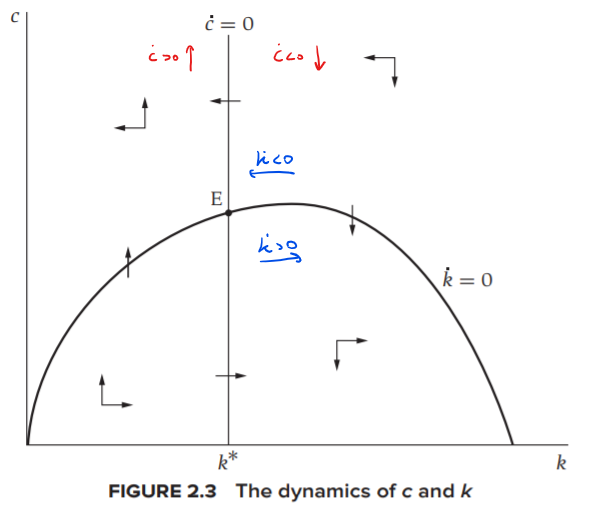
\includegraphics[width=0.45\linewidth]{subfile/attachments/2.1-dynamics of c and k.png}
            \end{subfigure}
            \begin{subfigure}
                \centering 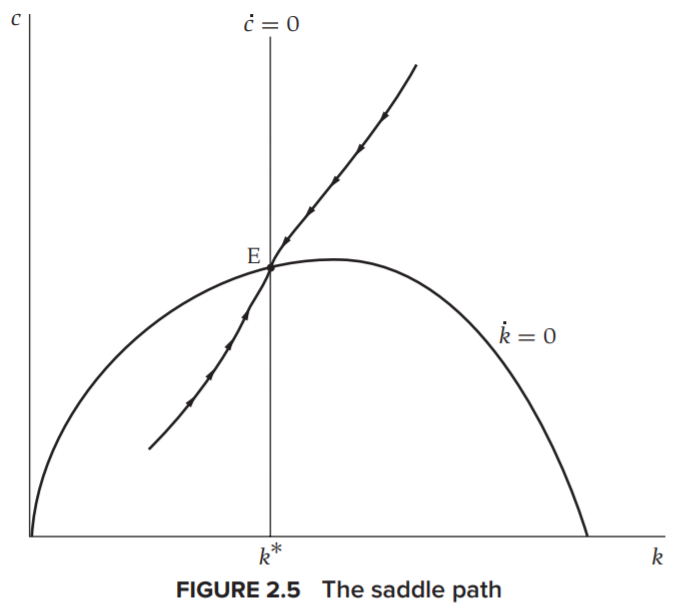
\includegraphics[width=0.45\linewidth]{subfile/attachments/2.2-saddle path.png}
            \end{subfigure}
        \end{figure}
        
        \vspace{0.5cm}
        
        We can also see effects of changes to other parameters, for example the discount rate
        \begin{align}
            \frac{\partial \dot c(t)}{\partial \rho} = -\frac{1}{\theta} < 0,
            \quad
            \frac{\partial \dot{k}(t)}{\partial \rho} = 0,
        \end{align}
        which implies a fall in discount rate $\rho$ will positively shift the locus of $k^*$ where $\dot c = 0$ while the $\dot k = 0$ path remains unchanged.
        
    \subsection{Derivations that $\dot c(t) = 0$ and $\dot k(t) = 0$ on the BGP}
    
        To see why $\frac{\dot c(t)}{c(t)} = 0$ on the BGP, let $g_c(t) = \frac{\dot c(t)}{c(t)}$. On the BGP, for $g_c(t)$ to be constant we must have that $\dot g_c(t) = 0$ and the second time derivative of consumption $\frac{d^2 c(t)}{dt} = \ddot c(t) = 0$. \? Then we have that on the BGP:
        % \begin{align}
        %     g_c
        %     &= \frac{\dot c}{c}
        %     = \frac{f'(k) - \rho - \theta g}{\theta}
        %     \\
        %     \implies
        %     \frac{\dot g_c}{g_c}
        %     &= \frac{d}{dt} [\ln (f'(k) - \rho - \theta g) + \ln \theta]
        %     = 0
        %     \\
        %     &= \frac{d \ln(f'(k) - \rho - \theta g)}{d f'(k)} \frac{d f'(k)}{dt}
        %     = \frac{f''(k)\dot k}{f'(k) - \rho - \theta g}
        %     = 0
        %     \\
        %     \implies
        %     \dot k &= 0
        % \end{align}
        \begin{align}
            \dot c(t)
            &= \frac{f'(k) - \rho - \theta g}{\theta} c(t)
            = g_c(t) c(t)
            \\
            \implies
            \ddot c(t)
            &= \dot g_c(t) c(t) +  g_c(t) \dot c(t) = 0
            \\
            \implies
            \frac{\dot c(t)}{c(t)}
            &= -\frac{\dot g_c(t)}{g_c(t)} = 0.
        \end{align}
        
        Then for capital on the BGP, the second time derivative $\ddot k(t) = 0$, and then:
        \begin{align}
            \ddot k(t)
            &= f'(k) \dot k(t) - \dot c(t) - (g+n) \dot k(t) = 0
            \implies
            \dot k(t) = \frac{\dot c(t)}{f'(k) - (g+n)} = 0.
        \end{align}
        
    \section{Golden-rule level of capital}\label{sec:RCK-GR}
        
        The \textbf{golden-rule level} capital stock $k_{GR}$ maximizes consumption $c(t)$. BGP capital stock $k^*$ in the RCK model will never exceed the golden-rule level $k_{GR}$. \\
        
        From \eqref{eqn:RCK-c-evo} we have that on the BGP
        \begin{align}
            f'(k^*) = \rho + \theta g.
        \end{align}
        
        From \eqref{eqn:RCK-k-evo} we get the golden-rule capital level $k_{GR}$, since when $\dot k = 0$ we have
        \begin{align}
            c = f(k) - (g + n)k,
            \quad
            \frac{\partial c}{\partial k} = 0 \implies
            f'(k_{GR}) = g + n.
        \end{align}
        
        We have from \eqref{eqn:rck-pv2} that $\beta = \rho - n - (1-\theta)g > 0$, then
        \begin{align}
            f'(k^*) - f'(k_{GR}) = \rho - n - (1-\theta)g > 0
            &\implies
            f'(k^*) > f'(k_{GR})
            \\
            &\implies
            k^* < k_{GR}
        \end{align}
        since $f'(k)$ is decreasing in $k$ ($f''(k) < 0$). Since $\beta > 0$, we have $k^* < k_{GR}$. However, $k^* \ge k_{GR}$ is possible in Solow growth model with sufficiently high savings rate.
    
    
    

\chapter{Diamond Model}
        
        Diamond model accounts for turnover of population. Technology and labor (population) follow laws of motion
        \begin{align}
            L_t = (1+n) L_{t-1},
            \quad
            A_t = (1+g) A_{t-1}
            \implies
            \frac{L_t}{L_{t+1}} = \frac{1}{1+n},
            \quad\frac{A_t}{A_{t+1}} = \frac{1}{1+n},
        \end{align}
        
        and capital follows law of motion
        \begin{align}
            K_{t+1} = (w_t A_t - C_{1, t} )L_t
        \end{align}
        
        where $W_t = w_t A_t$ is labor income and $C_{1,t}$ is consumption of young individuals at time $t$.
    
    
    \section{Firms}
    
        Similar to RCK model, firms production function and intensive are then
        \begin{align}    
            Y_t = F(K_t, A_t L_t),
            \quad
            y_t = \frac{Y_t}{A_t L_t}
            = F\left(\frac{K_t}{A_t L_t}, 1\right)
            = f(k_t) 
        \end{align}
        
        with
        \begin{align}
            r_t = f'(k_t),
            \quad
            w_t = \frac{W_t}{A_t}
            = f(k_t) - k_t f'(k_t),
        \end{align}
        
        which have the same derivations that result in \eqref{eqn:rck-eqm-interest} and \eqref{eqn:rck-eqm-wage}.
        
    
    \section{Households}
        
        Assume CRRA utility and that individuals live for two discrete periods. Let $C_{1, t}$ and $C_{2, t+1}$ be consumption of young and old individuals, individuals born in period $t$ maximizes lifetime utility
        \begin{align}
            \max_{C_{1, t}, C_{2, t+1}} U_t
            &= \frac{C_{1, t}^{1-\theta}}{1-\theta}
            + \frac{1}{1+\rho}
            \frac{C_{2, t+1}^{1-\theta}}{1-\theta},
            \quad \theta > 0,
            \quad \rho > -1.
            \label{eqn:diamond-pv}
            \\
            & s.t. \nonumber
            \\
            w_t A_t
            &= C_{1, t} + \frac{C_{2, t+1}}{1 + r_{t+1}}.
            \label{eqn:diamond-bc}
        \end{align}
        
        Form the Lagrangian
        \begin{align}
            \L
            = \frac{C_{1, t}^{1-\theta}}{1-\theta}
            + \frac{1}{1+\rho}
            \frac{C_{2, t+1}^{1-\theta}}{1-\theta}
            + 
            \lambda \left(
            w_t A_t
            - C_{1, t} - \frac{C_{2, t+1}}{1 + r_{t+1}}
            \right),
        \end{align}
        and with the first order conditions we have
        \begin{align}
            \frac{\partial \L}{\partial C_{1,t}} = 0
            &\implies
            C_{1, t}^{-\theta} = \lambda,
            \\
            \frac{\partial \L}{\partial C_{2,t+1}} = 0
            &\implies
            \frac{1}{1+\rho}C_{2, t+1}^{-\theta} = \frac{\lambda}{1+r_{t+1}}
        \end{align}
        
        Dividing the two FOC results gives us the \textbf{Euler equation} for consumption, which determines the optimal intertemporal choice:
        \begin{align}
            \frac{C_{2, t+1}}{C_{1, t}}
            = \left(\frac{1+r_{t+1}}{1+\rho}\right)^{1/\theta}.
            \label{eqn:diamond-euler}
        \end{align}
        
        Substituting back into the budget constraint \eqref{eqn:diamond-bc}, we have
        \begin{align}
            w_t A_t
            = C_{1, t} + \frac{1}{1+r_{t+1}} C_{2, t+1}
            &= C_{1, t} + \frac{1}{1+r_{t+1}} \left(\frac{1+r_{t+1}}{1+\rho}\right)^{1/\theta} C_{1, t}
            \\
            \implies
            w_t A_t
            &= \frac{
                (1+\rho)^{1/\theta} + (1+r_{t+1})^{(1-\theta)/\theta}}{
                (1+\rho)^{1/\theta}
                }
            C_{1, t}
            \\
            \implies
            C_{1, t}
            &=
            \frac{
                (1+\rho)^{1/\theta}
            }{
                (1+\rho)^{1/\theta} + (1+r_{t+1})^{(1-\theta)/\theta}
            }
                w_tA_t
        \end{align}
        
        Define savings rate $s(r)$ as
        \begin{align}
            s(r_{t+1})
            = \frac{w_t A_t - C_{1,t}}{w_t A_t}
            =\frac{
                (1+r_{t+1})^{(1-\theta)/\theta}
            }{
                (1+\rho)^{1/\theta} + (1+r_{t+1})^{(1-\theta)/\theta}
            },
        \end{align}
        which simplifies our consumption function:
        \begin{align}
            C_{1, t} = [1-s(r_{t+1})] w_t A_t.
        \end{align}
        
    \vspace{0.5cm}
    \section{Dynamics of model}
        
        We have for capital that
        \begin{align}
            K_{t + 1}
            &= (w_t A_t - C_{1, t})L_t
            = [s(r_{t+1})w_t A_t] L_t
            \\
            \implies
            k_{t+1} &= \frac{K_{t+1}}{A_{t+1} L_{t+1}} = s(r_{t+1})w_t \frac{A_t}{A_{t+1}}
            \frac{L_t}{L_{t+1}}
            =
            \frac{s(f'(k_{t+1}))}{(1+g)(1+n)}
            [f(k_t) - k_t f'(k_t)]
        \end{align}
        
        where $r_{t+1} = f'(k_{t+1})$ and $w(t) = f(k_t) - k_t f'(k_t)$.
        
        \vspace{0.5cm}
        
        On the balanced growth path, we have that $k_{t+1} = k_t = k^*$, where capital per effective labor becomes \textbf{globally stable across periods}. Consider the special case with Cobb-Douglas production $f(k) = k^\alpha$ and $\theta = 1$. We then have
        \begin{align}
            s(r_{t+1}) = \frac{1}{2+\rho}, \quad
            k_{t+1} = \frac{
                (1-\alpha) k_t^\alpha
            }{
                (1+g)(1+n)(2+\rho)
            }.
        \end{align}
        
        \begin{figure}[!ht]
            \centering
            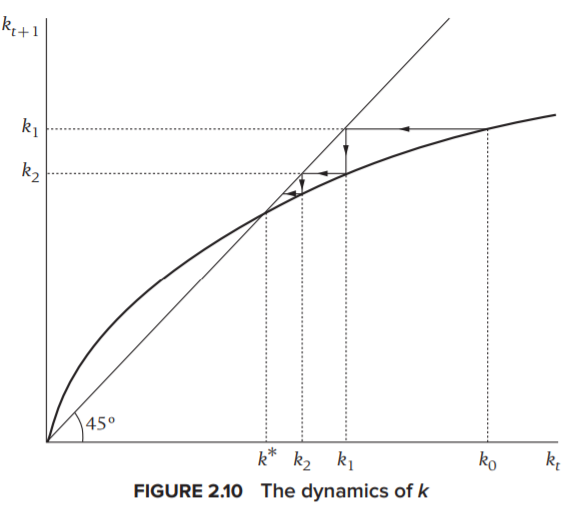
\includegraphics[width=0.65\textwidth]{subfile/attachments/2.3-diamond-k-evo.png}
        \end{figure}
        
        Effective capital will converge to $k^*$.
        
    \subsection{Dynamic inefficiency}
    
        \textbf{Dynamic inefficiency}, or Pareto inefficiency, is possible in the Diamond model if the equilibrium capital level exceeds the golden rule level $k^* > k_{GR}$. This this case consumption per worker can be increased in every generation if the capital is reduced to $k^* = k_{GR}$.
        
        \begin{figure}[ht!]
            \centering 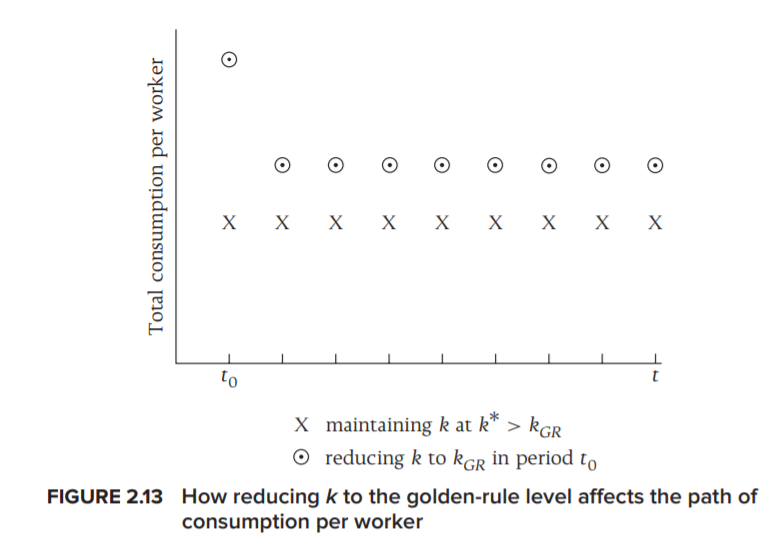
\includegraphics[width=0.75\textwidth]{subfile/attachments/2.5-diamond-dynamic-inefficiency.png}
        \end{figure}
        
        For RCK, dynamic inefficiency is not possible as the equilibrium capital level is always less than the golden rule level (see section \ref{sec:RCK-GR}). There would be a trade off in consumption between generations if BGP capital level was raised to golden rule.
        
\end{document}